\chapter{Implemetation and Evaluation}\label{ch:evaluation}

\section{Pilot Implementation}
% Все предложенные в данной работе подходы реализованы в созданном в рамках данной работы Хорн-решателе \theringen{} (\emph{R}egular \emph{In}variant \emph{Gen}erator)\footnote{\url{https://github.com/Columpio/RInGen}}.
% Реализация занимает 5200 строк на языке \fsharp{}.
% Было принято решение реализовать Хорн-решатель с нуля, не встраиваясь в кодовые базы существующих решателей, поскольку предложенные алгоритмы требуют нетривиальных манипуляций с формулами и результатами других логических решателей.
All the approaches proposed in this work have been implemented in a Horn solver \theringen{} (\emph{R}egular \emph{In}variant \emph{Gen}erator)\footnote{\url{https://github.com/Columpio/RInGen}}, which was developed as part of this thesis. The implementation comprises 5200 lines of \fsharp{} code. The decision was made to create a Horn solver from scratch, rather than integrating into the codebases of existing solvers, as the proposed algorithms require non-trivial manipulations of formulas and the results of other logical solvers.


% Общая архитектура реализованного инструмента представлена на рисунке~\ref{fig:ringen-arch}.
% Инструмент \theringen{} принимает на вход систему дизъюнктов Хорна с ограничениями в формате SMTLIB2~\cite{BarFT-RR-17}.
% После парсинга дизъюнктов выполняется их  упрощение, в частности, устранение равенств, селекторов и тестеров. Затем, в зависимости от поданных Хорн-решателю опций, запускается один из алгоритмов, предложенных в данной работе. Результатом работы каждого из них является формула над неинтерпретированными функциями, которая передаётся в сторонний логический решатель~--- \vampire{} или \cvc{}.
% В итоге инструмент возвращает безопасный индуктивный инвариант, если система безопасна, в противном случае~--- резолютивное опровержение.
The overall architecture of the tool is presented in Figure~\ref{fig:ringen-arch}.
\theringen{} takes as input a Horn clause system with constraints in the SMTLIB2 format~\cite{BarFT-RR-17}.
After the clauses are parsed, they are simplified, in particular, equalities, selectors, and testers are eliminated. Then, depending on the options submitted to the Horn solver, one of the algorithms proposed in this work is initiated. The output of each of these algorithms is a formula over uninterpreted functions, which is passed to an external logic solver~--- either \vampire{} or \cvc{}.
As a result, the tool returns a safe inductive invariant if the system is safe, otherwise, it returns a resolution refutation.

\begin{figure}[h]
% https://online.visual-paradigm.com/share.jsp?id=323637353533352d31
    \centering
    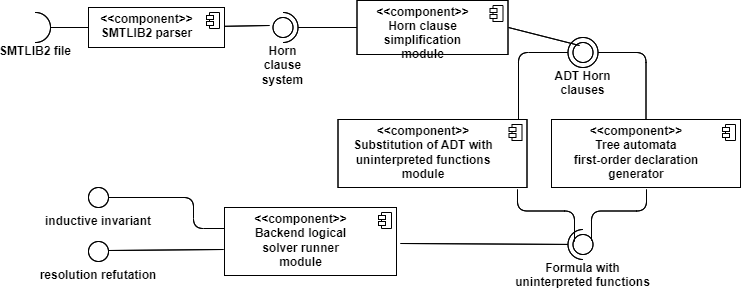
\includegraphics[width=\textwidth]{Dissertation/images/arch.png}
    \caption{Architecture of \theringen{}}
    \label{fig:ringen-arch}
\end{figure}


\textbf{\theringen{}.}\label{sec:ringen-pure}
% Итак, подход, представленный в главе~\ref{ch:fmf}, реализован автором данного исследования в рамках Хорн-решателя \theringen{}.
% Как сам подход, так и его реализация подразумевают использование стороннего SMT-решателя $\verifier$ для теории неинтерпретированных функций с кванторами, поэтому предлагаемая реализация в дальнейшем будет обозначаться $\ringen{\verifier}$.
% В частности, в качестве решателя $\verifier$ в экспериментах используются инструмент \vampire{}~\cite{reger2017instantiation} и SMT-решатель \cvc{}.
% Инструмент \vampire{} использует портфолио- подход~\cite{reger2014challenges}, то есть перебирает различные техники проверки выполнимости формул, построенные на насыщении системы~\cite{kovacs2013first} или на поиске конечных моделей~\cite{10.1007/978-3-319-40970-2_20}.
% Инструмент \cvc{} используется в режиме построения конечных моделей\footnote{с опцией \texttt{-{}-finite-model-find}}~\cite{reynolds2013finite}.
% Оба инструмента позволяют как доказывать безопасность системы, так и находить контрпримеры.
Hence, we implemented the approach presented in Chapter~\ref{ch:fmf} within the Horn solver \theringen{}. 
Both the approach itself and its implementation involve the use of an external SMT solver $\verifier$ for the theory of uninterpreted functions with quantifiers, therefore the proposed implementation will be further denoted as $\ringen{\verifier}$.
Specifically, \vampire{}~\cite{reger2017instantiation} and the SMT solver \cvc{} are used as the $\verifier$ in the experiments.
\vampire{} uses a portfolio-based approach~\cite{reger2014challenges}, that is, it iterates through various formula satisfiability checking techniques, based on saturation of the system~\cite{kovacs2013first} or finite model finding~\cite{10.1007/978-3-319-40970-2_20}.
\cvc{} is used in the finite model construction mode\footnote{with the \texttt{-{}-finite-model-find} option}~\cite{reynolds2013finite}.
Both tools allow for both proving the safety of the system and finding counterexamples.

\textbf{\ringenSync{}.}
% Этот подход представленный в  главе~\ref{ch:SyncReg}, реализован как надстройка над $\ringen{\verifier}$.
% В качестве стороннего решателя $\verifier$ в экспериментах использовался \cvc{}, поскольку \ringenSync{} порождает символы с большой арностью, которые не поддерживаются инструментом \vampire{}\footnote{\url{https://github.com/vprover/vampire/issues/348\#issuecomment-1091782513}}.
% Эта реализация в дальнейшем будет обозначаться \ringenSync{}\footnote{\url{https://github.com/Columpio/RInGen/releases/tag/ringen-tta}}.
The approach presented in Chapter~\ref{ch:SyncReg} has been implemented as an extension of $\ringen{\verifier}$.
In the experiments, \cvc{} was used as the external solver $\verifier$, as \ringenSync{} generates symbols with high arity, which are not supported by \vampire{}\footnote{\url{https://github.com/vprover/vampire/issues/348\#issuecomment-1091782513}}.
This implementation will be hereinafter referred to as \ringenSync{}\footnote{\url{https://github.com/Columpio/RInGen/releases/tag/ringen-tta}}.

\textbf{\theringenCICI{}.}
% Данный подход, представленный  в главе~\ref{ch:cici}, реализован в рамках кодовой базы Хорн-решателей \racer{}~\cite{10.1145/3498722} (развитие Хорн-решателя \spacer{}~\cite{komuravelli2016smt}, реализованное в логическом решателе \zprover{}\footnote{\url{https://github.com/Columpio/z3/tree/racer-solver-interaction}}) и Хорн-решателя $\ringen{\verifier{}}$\footnote{\url{https://github.com/Columpio/RInGen/releases/tag/chccomp22}}, описанного выше.
% Эта реализация в дальнейшем будет обозначаться $\ringenCICI{\verifier{}}$. Далее описаны обе части этой реализации в Хорн-решателях \racer{} и $\ringen{\verifier{}}$, соответственно, которые далее называются \emph{базовыми} относительно инструмента $\ringenCICI{\verifier{}}$.
The approach presented in Chapter~\ref{ch:cici} has been implemented within the codebase of the Horn solvers \racer{}\cite{10.1145/3498722} (a development of the Horn solver \spacer{}\cite{komuravelli2016smt}, implemented in the logical solver \zprover{}\footnote{\url{https://github.com/Columpio/z3/tree/racer-solver-interaction}}) and the Horn solver $\ringen{\verifier{}}$\footnote{\url{https://github.com/Columpio/RInGen/releases/tag/chccomp22}}, which was described earlier.
This implementation will be referred to as $\ringenCICI{\verifier{}}$ in the future. The following describes both parts of this implementation in the Horn solvers \racer{} and $\ringen{\verifier{}}$, respectively, which are subsequently referred to as \emph{basic} relative to the tool $\ringenCICI{\verifier{}}$.


\paragraph{\zprover{}/\racer{}.}
% Хорн-решатель \racer{} разработан Ари Гурфинкелем (Arie Gurfinkel) и Хари Говинд Ведирамана Кришнаном (Hari Govind Vediramana Krishnan) из университета Ватерлоо.
% Инструмент \racer{} основан на подходе, называемом достижимость, направляемая свойством (Property-Directed Reachability, PDR)~\cite{komuravelli2016smt}, который можно рассматривать как сложный экземпляр \cegar{}.
% PDR строит абстрактные состояния в виде конъюнкции формул (называемых \emph{леммами}) на различных \emph{уровнях} путём итеративного увеличения уровня в цикле.
% При этом поддерживаются следующие возможности: если набор лемм $\{\phi_i\}$ был построен на уровне $n$, то $\bigwedge_i \phi_i$ аппроксимирует сверху все состояния, достижимые менее чем за $n$ шагов перехода, и аппроксимирует снизу свойство безопасности.
% Таким образом, леммы в PDR выполняют требование абстракции в процедуре \RunBlackBox{} (алгоритм~\ref{code:runblackbox}).
% Хорн-решатель \racer{} был модифицирован в рамках данного диссертационного исследования таким образом, чтобы в конце каждой итерации набор лемм последнего уровня асинхронно передавался новому процессу инструмента $\ringen{\verifier{}}$.
The \racer{} Horn solver was developed by Arie Gurfinkel and Hari Govind Vediramana Krishnan from the University of Waterloo. It is based on an approach called Property-Directed Reachability (PDR)~\cite{komuravelli2016smt}, which can be considered a complex instance of \cegar{}. PDR builds abstract states in the form of conjunctions of formulas (referred to as \emph{lemmas}) at various \emph{levels} by iteratively increasing the level in a loop. The following capabilities are supported: if a set of lemmas $\{\phi_i\}$ was constructed at level $n$, then $\bigwedge_i \phi_i$ over-approximates all states reachable in less than $n$ transition steps, and under-approximates the safety property. Thus, in PDR, lemmas fulfill the requirement of abstraction in the \RunBlackBox{} procedure (algorithm~\ref{code:runblackbox}). As part of this thesis, \racer{} was modified to asynchronously pass the set of lemmas from the last level to a new process of $\ringen{\verifier{}}$ at the end of each iteration.


\paragraph{$\ringen{\verifier{}}$.}
% Процедура \RunBlackBox{} (алгоритм~\ref{code:runblackbox}) реализована на основе инструмента  $\ringen{\verifier{}}$. Было выполнено  следующее обобщение в процедуре $\substituteLemmas(\prog, a)$ (см.~\autoref{sec:subst_lemmas}).
% Конъюнктивная форма лемм инструмента \racer{} используется для вывода инвариантов более общего вида:
% $\bigwedge_i(\phi_i(\overline{x})\,\lor\,\overline{x}\!\in\!L_i)$.
% Так, имея $a(P) = \bigwedge_i \phi_i$,
% мы заменяем все атомы $P(\overline{t})$ на \emph{конъюнкцию дизъюнкций} $\bigwedge_i (\phi_i(\overline{t})\lor L_i(\overline{t}))$ с новыми предикатными символами $L_i$.
% Это позволяет выводить более общие инварианты, чем инварианты из объединения классов $\elemclass{}$ и $\abstrDomain$ (см. определение~\ref{def:combined-class}), которое состоит только из формул вида $\phi(\overline{x})\,\lor\,\overline{x}\!\in\!L$.
The \RunBlackBox{} procedure (algorithm~\ref{code:runblackbox}) is implemented based on the $\ringen{\verifier{}}$. The following generalization was carried out in the $\substituteLemmas(\prog, a)$ procedure (see~\autoref{sec:subst_lemmas}). The conjunctive form of lemmas from \racer{} is used to infer more general invariants: $\bigwedge_i(\phi_i(\overline{x})\,\lor\,\overline{x}\!\in\!L_i)$. Hence, given $a(P) = \bigwedge_i \phi_i$, we replace all atoms $P(\overline{t})$ with a \emph{conjunction of disjunctions} $\bigwedge_i (\phi_i(\overline{t})\lor L_i(\overline{t}))$ with new predicate symbols $L_i$. This allows inferring more general invariants than those from the union of $\elemclass{}$ and $\abstrDomain$ (see Definition~\ref{def:combined-class}), which consists only of formulas of the form $\phi(\overline{x})\,\lor\,\overline{x}\!\in\!L$.

% После преобразований модифицированный $\ringen{\verifier{}}$ вызывает сторонний решатель $\verifier{}$ с ограничением по времени в 30 секунд.
% Затем его результаты передаются обратно в Хорн-решатель \racer{}, где они асинхронно обрабатываются.
% Кроме того, реализация не выполняет дорогостоящее преобразование в КНФ из алгоритма~\ref{code:residual-chc}, так как реализация $\ringen{\verifier{}}$ позволяет принимать на вход дизъюнкты Хорна в произвольном виде, поскольку он полагается на сторонний решатель $\verifier{}$ с полной поддержкой логики первого порядка.
After the transformations, the modified $\ringen{\verifier{}}$ calls the external solver $\verifier{}$ with a time limit of 30 seconds. Then its results are passed back to \racer{}, where they are processed asynchronously. Moreover, the implementation does not perform the costly transformation into CNF from algorithm~\ref{code:residual-chc}, as the $\ringen{\verifier{}}$ implementation allows inputting Horn clauses in arbitrary form, since it relies on the external solver $\verifier{}$ with full first-order logic support.


\section{Evaluation}
\subsection{Tool Selection}
% В качестве инструментов для сравнения были выбраны \racer{}~\cite{10.1145/3498722} и \eldarica{}~\cite{8603013}~--- Хорн-решатели с поддержкой алгебраических типов данных, лидирующие на соревнованиях \chccomp{}~\cite{De_Angelis_2022}.
% Также  были выбраны инструменты \cvcind{} (\cvc{} в режиме индукции)~\cite{reynolds2015induction} и \vericat{}~\cite{10.1093/logcom/exab090}.
% Несмотря на то, что эти инструменты не строят индуктивные инварианты \emph{явно}, из-за чего невозможно проверить их корректность, их запуск на эквивалентном бенчмарке добавлен в экспериментальное сравнение, поскольку они решают родственную задачу.
We have selected the \racer{}~\cite{10.1145/3498722} and \eldarica{}~\cite{8603013} tools for compassion, which are Horn solvers with support for algebraic data types leading in the \chccomp{} competition~\cite{De_Angelis_2022}. We also selected \cvcind{} (\cvc{} in induction mode)~\cite{reynolds2015induction} and \vericat{}~\cite{10.1093/logcom/exab090}. Although these tools do not construct inductive invariants explicitly, making it impossible to check their correctness, their launch on an equivalent benchmark is added to the experimental comparison as they solve a related task.


% В представленных здесь экспериментах не участвовал Хорн-решатель \hoice{}~\cite{10.1007/978-3-030-02768-1_8}, поскольку он работает не быстрее \racer{}~\cite{10.1145/3498722} и при этом ищет инварианты в том же классе инвариантов \elemclass{}.
% Другой известный Хорн-решатель \rchc{}~\cite{haude2020} не участвовал в экспериментах, поскольку он работает нестабильно и  часто либо завершается с ошибкой, либо возвращает некорректные результаты.

\subsection{Benchmark Suite}
% Эксперименты проводились на наборе данных \emph{TIP} (Tons of Inductive Problems)~\cite{claessen2015tip}, тестового набора с трека соревнования \chccomp{} 2022\footnote{\url{https://github.com/chc-comp/ringen-adt-benchmarks}}, посвящённого алгебраическим типам данных. Набор \emph{TIP} состоит из 454 систем дизъюнктов Хорна, полученных из \haskell{}-программ с АТД и рекурсией.
% В тестовом наборе встречаются следующие алгебраические типы данных~--- списки, очереди, регулярные выражения и целые числа Пеано.

The experiments were conducted on the TIP (Tons of Inductive Problems) benchmark suite~\cite{claessen2015tip}, the test set from the 2022 \chccomp{} competition track\footnote{\url{https://github.com/chc-comp/ringen-adt-benchmarks}}, dedicated to algebraic data types. The TIP set consists of 454 Horn clause systems derived from Haskell programs with ADTs and recursion. The test set includes the following algebraic data types: lists, queues, regular expressions, and Peano integers.

\subsection{Setup}
% Эксперименты проводились на платформе StarExec~\cite{stump2014starexec}, имеющей кластер машин с Intel(R) Xeon(R) CPU E5-2609 0 @ 2.40GHz и Red Hat Enterprise Linux~7\footnote{\url{https://www.starexec.org/starexec/public/machine-specs.txt}}, с ограничением на процессорное время работы каждого инструмента на каждом тесте в 600~секунд и с ограничением по памяти в 16~ГБ.
The experiments were conducted on the StarExec platform~\cite{stump2014starexec}, which has a cluster of machines with Intel(R) Xeon(R) CPU E5-2609 0 @ 2.40GHz and Red Hat Enterprise Linux~7\footnote{\url{https://www.starexec.org/starexec/public/machine-specs.txt}}, with a limit on the CPU runtime for each tool on each test of 600 seconds and a memory limit of 16 GB.

\subsection{Research Questions}

% Для постановки экспериментов были поставлены следующие исследовательские вопросы.
We have formulated the following research questions to guide the experimental setup.
\begin{resquest}[Number of solutions]\label{rq:conv}
$ $

% Поскольку основная цель данной работы~--- предложить подходы, позволяющие проверять выполнимость б\textit{о}льшего числа систем, чем аналоги, путём вывода индуктивных инвариантов, ключевыми являются следующие вопросы.
\begin{itemize}
    % \item Позволяют ли предложенные подходы проверять выполнимость б\textit{о}льшего числа систем, чем подходы, строящие классические символьные инварианты?
    % \item Позволяют ли предложенные подходы проверять выполнимость систем, у которых существуют классические инварианты?
    \item Do the proposed methods allow for the verification of more systems than approaches that construct classical symbolic invariants?
    \item Do the proposed methods allow for the verification of systems that have classical invariants?

\end{itemize}
\end{resquest}

\begin{resquest}[Performance]\label{rq:perf}
$ $

\begin{itemize}
    % \item Какова производительность инструментов \theringen{} и \ringenSync{} на проблемах, которые смогли решить они, а также существующие инструменты?
    % \item Коллаборативный вывод в \theringenCICI{} может потребовать параллельного запуска нескольких экземпляров оракула. Каково влияние параллельного запуска на производительность?
    \item What is the performance of \theringen{} and \ringenSync{} on problems that they, as well as existing tools, were able to solve?
    \item Collaborative inference in \theringenCICI{} may require parallel launching of multiple oracle instances. What is the impact of parallel launching on performance?

\end{itemize}
\end{resquest}

\begin{resquest}[Significance of the inductive invariant class]\label{rq:char}
$ $

% Коллаборативный вывод, реализованный в \theringenCICI{}, теоретически позволяет не только выводить инварианты в большем классе, но и ускорять сходимость поиска классических символьных инвариантов. Какова при этом доля классических символьных инвариантов на всех уникально решённых инструментом \theringenCICI{} проблемах?
Collaborative inference, implemented in \theringenCICI{}, theoretically allows not only to infer invariants in a larger class but also to accelerate the convergence of the search for classical symbolic invariants. What is the share of classical symbolic invariants in all uniquely solved problems by \theringenCICI{}?
\end{resquest}



\section{Results}



\subsection{Number of Solutions}

% Количество проблем из тестового набора, решённых существующими и предложенными инструментами, представлено в таблице~\ref{table:eval-all}.
The number of problems from the benchmark suite solved by the existing and proposed instruments is presented in Table~\ref{table:eval-all}.
\begin{table}[t]
    \caption{Results. SAT indicates that the system is safe (there is an inductive invariant), UNSAT indicates that the system is unsafe.}
    \label{table:eval-all}
    \small
    \centering
    \begin{tabular}{ |l|c|c| }
    \hline
    Tool & SAT & UNSAT\\\hline
    \cvcind{} & 0 & 13\\
    \eldarica{} & 46 & 12\\
    \racer{} & 26 & 22\\
    \ringen{\cvc{}} & 25 & 21\\
    \ringen{\vampire{}} & 135 & 46\\
    \ringenCICI{\cvc{}} & 117 & 19\\
    \ringenCICI{\vampire{}} & 189 & 28\\
    \ringenSync{} & 43 & 21\\
    \vericat{} & 16 & 10\\
    \hline
    \end{tabular}
\end{table}

%\subsubsection{\theringen{}.}

% \textbf {\theringen{}}. На всех 12 проблемах, на которых инструмент \eldarica{} вернул ответ <<UNSAT>>, инструмент \theringen{} завершился с тем же результатом и он нашёл больше контрпримеров.
% Инструменты \ringen{\cvc{}}, \ringen{\vampire{}} и \racer{} нашли контрпримеры для 21, 46 и 22 систем дизъюнктов соответственно. Большинство из этих систем совпадает, хотя некоторые из них уникальны для каждого инструмента.
% Инструмент \ringen{\vampire{}} построил существенно больше <<UNSAT> результатов, чем другие инструменты, поскольку в инструменте \vampire{} реализована эффективная процедура вывода опровержений.
% Тем самым, несмотря на то, что предложенные алгоритмы спроектированы для поиска большего числа индуктивных инвариантов, они также позволяют находить уникальные контрпримеры.
% Далее, инструмент \eldarica{} нашёл 46 инвариантов в противовес 25 и 135 инвариантам, найденным \ringen{\cvc{}} и \ringen{\vampire{}}.
% Из них \eldarica{} решила 25 уникальных (не решённых \ringen{\cvc{}}) задач, каждая из которых является формулировкой некоторого свойства порядковых предикатов ($ <, \le,>, \ge $) на числах Пеано.
% Эти проблемы легко решаются инструментом \eldarica{}, поскольку порядковые предикаты сами по себе включены в домен верификации \sizeelemclass{} на уровне примитивов.
% Тем не менее инструмент \ringen{\cvc{}} решил 13 уникальных (не решённых \eldarica{}) проблем, чьи инварианты не представимы в домене верификации инструмента \eldarica{}.
% Эффективность реализованного в инструменте \theringen{} подхода существенно зависит от используемого стороннего решателя, как видно из того, что инструмент \ringen{\vampire{}} вывел более чем в 5 раз больше инвариантов, чем инструмент \ringen{\cvc{}}.
\textbf{\theringen{}}. On all 12 problems where \eldarica{} returned UNSAT, \theringen{} terminated with the same result, and it found more counterexamples.
The \ringen{\cvc{}}, \ringen{\vampire{}}, and \racer{} found counterexamples for 21, 46, and 22 clause systems, respectively. Most of these systems are the same, although some are unique to each tool.
\ringen{\vampire{}} constructed significantly more UNSAT results than other tools, as \vampire{} implements an efficient refutation inference procedure.
Therefore, even though the proposed algorithms are designed to search for more inductive invariants, they also allow for finding unique counterexamples.
Next, \eldarica{} found 46 invariants in contrast to 25 and 135 invariants found by \ringen{\cvc{}} and \ringen{\vampire{}}.
Out of these, \eldarica{} solved 25 unique (not solved by \ringen{\cvc{}}) tasks, each of which is a formulation of some property of ordinal predicates ($ <, \le,>, \ge $) on Peano numbers.
These problems are easily solved by \eldarica{}, as ordinal predicates are themselves included in the \sizeelemclass{} verification domain at the primitive level.
However, \ringen{\cvc{}} solved 13 unique (not solved by \eldarica{}) problems, which invariants are not expressible in the verification domain of the \eldarica{}.
The effectiveness of the approach implemented in the \theringen{} heavily depends on the external solver used, as evidenced by the fact that \ringen{\vampire{}} inferred more than 5 times more invariants than \ringen{\cvc{}}.


% \textbf{\ringenSync{}.} Данный инструмент завершился с ответом UNSAT на 21 проблеме, эти ответы в точности совпадают с 21 результатом инструмента \ringen{\cvc{}}, поскольку поиск контрпримеров инструмент \ringenSync{} наследует от последнего.
\textbf{\ringenSync{}.} This tool terminated with UNSAT on 21 problems, these results exactly match the 21 results of the \ringen{\cvc{}}, since \ringenSync{} inherits the counterexample search from the latter.

% Среди всех полученных инструментом \eldarica{} ответов SAT 38 были также получены инструментом \ringenSync{}.
% Большое количество пересечений с результатами инструмента \eldarica{} связано с тем, что \eldarica{} хорошо справляется с проблемами, которые кодируют порядок на числах Пеано, который также хорошо кодируется полносвёрточными синхронными автоматами над деревьями, используемыми в \ringenSync{}. \racer{} завершился с ответом SAT на 26 системах, 15 из которых пересекаются с ответами инструмента \ringenSync{}. Также инструмент \ringenSync{} вывел 4 уникальных инварианта. Несмотря на то, что теоретически выразительная сила полносвёрточных синхронных автоматов над деревьями, используемых в \ringenSync{}, должна давать большее число решений, инструменты поиска конечных моделей, которые \ringenSync{} использует в качестве бэкенда, не завершаются на проблемах с большим количеством кванторов и потому \ringenSync{} часто не завершается.
% Результаты не меняются при изменении бэкенда с \cvc{} на другие инструменты поиска конечных моделей и увеличении ограничения на время до 1200 секунд. Небольшое количество пересечений с инструментом \racer{} говорит о том, что хотя в теории класс элементарных инвариантов почти полностью содержится в классе синхронных регулярных инвариантов, на практике предложенный подход не позволяет эффективно выводить инварианты систем, у которых существуют элементарные инварианты.
Among all SAT results obtained by \eldarica{}, 38 were also obtained by \ringenSync{}.
The large overlap with the results of \eldarica{} is due to the fact that \eldarica{} deals well with problems encoding the order on Peano numbers, which are also well-encoded by the fully-convolutional synchronous tree automata used in \ringenSync{}. \racer{} concluded with a SAT result on 26 systems, 15 of which intersect with the results of \ringenSync{}. Additionally, \ringenSync{} inferred 4 unique invariants. Despite the theoretical expressive power of the fully-convolutional synchronous tree automata used in \ringenSync{}, which should yield a larger number of solutions, the finite model finding tools that \ringenSync{} uses as a backend do not terminate on problems with a large number of quantifiers, and therefore \ringenSync{} often does not terminate.
The results do not change when changing the backend from \cvc{} to other finite model finding tools and increasing the time limit to 1200 seconds. The small overlap with \racer{} suggests that although in theory the class of elementary invariants is almost fully contained in the class of synchronous regular invariants, in practice the proposed approach does not effectively infer invariants of systems that have elementary invariants.


% \textbf{\theringenCICI{}.} Инструмент \theringenCICI{} решил меньше \textit{небезопасных проблем}, чем лучший из базовых решателей: \theringenCICI{} получил 19 (с \cvc{}) и 28 (с \vampire{}) UNSAT результатов против 21 (с \cvc{}) и 46 (с \vampire{}) UNSAT результатов, полученных \theringen{}. Основная причина в том, что предложенный подход спроектирован для решения более сложной задачи вывода индуктивных инвариантов и не вносит изменения в работу базовых алгоритмов поиска контрпримеров. То есть, с нашим подходом могут быть интегрированы ортогональные усовершенствования поиска контрпримеров, например, предложенные в~\cite{blicha2022transition}. Таким образом, все контрпримеры, полученные \theringenCICI{}, получены непосредственно от одного из базовых решателей. Некоторые контрпримеры, которые находит инструмент \theringen{}, не были найдены \theringenCICI{}, поскольку он запускает \theringen{} с ограничением по времени в 30 секунд. 
\textbf{\theringenCICI{}.} \theringenCICI{} solved fewer \textit{unsafe problems} than the best of the basic solvers: \theringenCICI{} obtained 19 (with \cvc{}) and 28 (with \vampire{}) UNSAT results against 21 (with \cvc{}) and 46 (with \vampire{}) UNSAT results obtained by \theringen{}. The main reason is that the proposed approach is designed to solve the more complex task of inferring inductive invariants and does not change the operation of the basic counterexample finding algorithms. That is, our approach can be integrated with orthogonal improvements to counterexample search, for example, those proposed in~\cite{blicha2022transition}. Thus, all counterexamples obtained by \theringenCICI{} are directly obtained from one of the basic solvers. Some counterexamples found by \theringen{} were not found by \theringenCICI{}, as it runs \theringen{} with a time limit of 30 seconds.

% Важно отметить, что все 20 SAT и 15 UNSAT ответов, полученных \racer{}, также были получены и инструментом \theringenCICI{}, за исключением одного UNSAT ответа.
It is important to note that all 20 SAT and 15 UNSAT answers obtained by \racer{}, were also obtained by \theringenCICI{}, with the exception of one UNSAT answer.

% \textit{На безопасных проблемах} инструмент \theringenCICI{} превзошёл конкурирующие решатели: \ringenCICI{\cvc{}} получил 117 SAT ответов, когда как \racer{} получил 20 SAT ответов, а \ringen{\cvc{}}~--- 25, также \ringenCICI{\vampire{}} получил 189 SAT ответов, при 20 SAT ответах от \racer{} и 135 от \ringen{\vampire{}}. 
% Таким образом, \theringenCICI{} решает значительно больше SAT задач, чем базовые инструменты, работающие по отдельности: 117 против $20+25$ и 189 против $20+135$ для соответствующих бэкендов \cvc{} и \vampire{}.
% В частности, \ringenCICI{\cvc{}} решает 97 задач, не решённых \racer{} и 94 задачи, не решённые \ringen{\cvc{}}.
% \ringenCICI{\vampire{}} решает 169 задач, не решённых \racer{} и 60 задач, не решённых \ringen{\vampire{}}.
% Таким образом, коллаборативный метод вывода инвариантов позволяет установить выполнимость существенно больше числа систем, чем параллельный запуск базовых инструментов.
\textit{On safe problems}, \theringenCICI{} outperformed competitive solvers: \ringenCICI{\cvc{}} obtained 117 SAT responses, while \racer{} obtained 20 SAT responses, and \ringen{\cvc{}} 25. \ringenCICI{\vampire{}} obtained 189 SAT responses, with 20 SAT responses from \racer{} and 135 from \ringen{\vampire{}}.
Thus, \theringenCICI{} solves significantly more SAT tasks than the basic tools working separately: 117 versus $20+25$ and 189 versus $20+135$ for the respective \cvc{} and \vampire{} backends.
In particular, \ringenCICI{\cvc{}} solves 97 tasks not solved by \racer{} and 94 tasks not solved by \ringen{\cvc{}}.
\ringenCICI{\vampire{}} solves 169 tasks not solved by \racer{} and 60 tasks not solved by \ringen{\vampire{}}.
Therefore, the collaborative invariant inference method allows to establish the feasibility of significantly more systems than the parallel launch of basic tools.

% Однако есть проблемы, которые были решены базовыми решателями, но не предложенным инструментом. Инструмент \ringenCICI{\cvc{}} не решил 7 проблем, которые были успешно решены инструментом \ringen{\cvc{}}. Две из этих проблем могут быть решены предложенным инструментом, если увеличить 30-секундное ограничение по времени для работы бэкенда в \theringenCICI{}. Существующие методы предсказания времени проверки, такие как~\cite{10.1145/3121257.3121262}, могут быть применены для того, чтобы вообще избежать жесткого кодирования лимита времени. Остальные 5 проблем решаются мгновенно, однако их результаты не могут быть получены из межпроцессного взаимодействия в сделанной реализации. Причина заключается в том, что \racer{} тратит слишком большое время на решение SMT-ограничений, и поэтому не считывает результаты бэкенд-решателя. Этой технической проблемы можно избежать, если считывать результаты бэкенд-решателя в более частых контрольных точках, что, однако, приведёт к увеличению накладных расходов в инструменте. Аналогичная картина наблюдается и для \ringenCICI{\vampire{}}, который не смог решить 24 проблемы, решённые базовыми решателями. Только 8 из них не решены из-за низкого ограничения по времени для бэкенда, а остальные 16~--- из-за расхождения \racer{} в решении SMT-ограничений.
However, there are problems that were solved by the basic solvers but not by the proposed tool. \ringenCICI{\cvc{}} did not solve 7 problems that were successfully solved by \ringen{\cvc{}}. Two of these problems could be solved by the proposed tool if the 30-second time limit in \theringenCICI{} was increased. Existing methods of prediction of verification time, such as~\cite{10.1145/3121257.3121262}, can be applied to avoid hard-coding a time limit at all. The remaining 5 problems are solved instantly, but their results cannot be retrieved from the inter-process interaction in the implemented solution. The reason is that \racer{} spends too much time solving SMT constraints and therefore does not read the results of the backend solver. This technical issue can be avoided by reading the results of the backend solver at more frequent checkpoints, which, however, will result in an increase in overhead in the tool. A similar situation is observed for \ringenCICI{\vampire{}}, which failed to solve 24 problems solved by the basic solvers. Only 8 of them are unsolved due to the low time limit for the backend, while the remaining 16 are due to \racer{} divergence in solving SMT constraints.

% Итак, инструмент \ringen{\cvc{}} не опередил существующие решения, однако дал множество уникальных решений по сравнению с ними, поскольку выводил инварианты в новом классе. Инструмент \ringen{\vampire{}}, построенный на том же подходе, решил более чем в 2.5 раза больше проблем, чем лучший из существующих инструментов, по той же причине. Несмотря на то, что класс инвариантов инструмента \ringenSync{} существенно шире, вывод инвариантов в нём гораздо более трудоёмкий, поэтому хотя он смог вывести почти в два раза больше инвариантов, чем \ringen{\cvc{}}, он не превзошёл лучший из существующих инструментов. Лучшие результаты показал инструмент \ringenCICI{\cvc{}}, который решил на 235\% больше задач, чем параллельная композиция \racer{} и \ringen{\cvc{}}, а также на 39\% больше задач c бэкендом \vampire{}, благодаря балансу между размером класса инвариантов и эффективностью процедуры вывода инвариантов. Наилучший из предложенных инструментов \ringenCICI{\vampire{}} всего решил $189+28$ проблем, что примерно в 3.74 раза больше, чем наилучший из существующих инструментов \eldarica{}, решивший $46+12$ проблем.

Therefore, \ringen{\cvc{}} did not outperform the existing solutions, but it did provide many unique solutions compared to them, as it inferred invariants in a new class. \ringen{\vampire{}} , built on the same approach, solved over 2.5 times more problems than the best of the existing tools, for the same reason. Despite the fact that the class of invariants of \ringenSync{} is significantly broader, inferring invariants in it is much more labor-intensive, so although it was able to infer almost twice as many invariants as \ringen{\cvc{}}, it did not outperform the best of the existing tools. The best results were shown by \ringenCICI{\cvc{}}, which solved 235\% more tasks than the parallel composition of \racer{} and \ringen{\cvc{}}, and also 39\% more tasks with the \vampire{} backend, thanks to the balance between the size of the class of invariants and the efficiency of the invariant inference procedure. The best of the proposed tools, \ringenCICI{\vampire{}}, solved a total of $189+28$ problems, which is about 3.74 times more than the best of the existing tools, \eldarica{}, which solved $46+12$ problems.

\subsection{Performance}\label{sec:evaluation/performance}

\toolplotOne{}

% Графики на рисунке~\ref{fig:toolplotOne} показывают, что инструмент \ringen{\cvc{}} не только выводит больше инвариантов, но и работает быстрее, чем другие инструменты, в среднем, на один порядок. На рисунке некоторые небезопасные системы проверялись быстрее инструментами \cvcind{}, \vericat{} и \racer{}. Это может быть связано с более эффективной процедурой инстанцирования кванторов в \cvcind{} и более сбалансированным компромиссом между выводом инвариантов и поиском контрпримеров в ядре \racer{} (который также вызывается инструментом \vericat{}).
% На проблемах, решённых несколькими инструментами, инструмент \ringen{\cvc} работает в среднем на два порядка быстрее.
% Запуски \ringen{\vampire{}} заняли ещё меньше времени, чем \ringen{\cvc}.
The plots in Figure~\ref{fig:toolplotOne} show that \ringen{\cvc{}} not only infers more invariants but also works faster than the other tools, on average, by one order of magnitude. In the figure, some unsafe systems were checked faster by \cvcind{}, \vericat{}, and \racer{}. This may be associated with a more efficient quantifier instantiation procedure in \cvcind{} and a more balanced trade-off between invariant inference and counterexample search in the core of \racer{} (which is also called by \vericat{}).
On problems that were solved by several tools, the \ringen{\cvc} operates on average two orders of magnitude faster.
The \ringen{\vampire{}} runs took even less time than \ringen{\cvc}.

\begin{figure}
    \pgfplotsset{width=1.\textwidth,height=0.3\textheight}
    \pgfplotstablegetrowsof{Dissertation/images/overhead.csv}
    \pgfmathsetmacro\NRows{\pgfplotsretval}
        \centering
    \begin{tikzpicture}
    \begin{axis}[
        ybar interval,
        ymin=0,
        ymax=20,
        xticklabel={\pgfmathprintnumber\tick-\pgfmathprintnumber\nexttick\%},
        % xticklabel={$\sim$\pgfmathparse{(\tick+\nexttick)/2}\pgfmathprintnumber{\pgfmathresult}\%},
        yticklabel={\pgfmathprintnumber\tick},
    ]
    \addplot +[
        hist={
            bins=8,
            data min=0.0,
            data max=80.0
        }
    ] table [y index=0] {Dissertation/images/overhead.csv};
    \end{axis}
    \end{tikzpicture}\caption{ Number of benchmark instances (y-axis) solved by both \theringenCICI{} and \racer{}, and the CPU time overhead (x-axis) of running \theringenCICI{} compared to \racer{}. \racer{} outperforms \theringenCICI{} on 34 instances. There are no instances with an overhead larger than 80\%, so the x-axis is not shown further.}
    %Количество тестовых примеров (ось y), решённых как \theringenCICI{}, так и \racer{}, и затраты процессорного времени (ось абсцисс) на выполнение \theringenCICI{} по сравнению с \racer{}. \racer{} превзошел \theringenCICI{} на 34 запусках. Нет ни одного запуска с накладными расходами более 80\%, поэтому далее ось абсцисс не показана.}
    \label{fig:performance}
\end{figure}

\begin{figure*}
\toolplotTwo{\cvc{}}{Dissertation/images/toolplot_cvc.csv}
~
\toolplotTwo{\vampire{}}{Dissertation/images/toolplot_vampire.csv}
\caption{Runtime comparison}
\label{fig:toolplot}
\end{figure*}

% \textbf{\ringenSync{} и \theringenCICI{} }. На рисунке~\ref{fig:toolplot} представлены \textit{общие графики производительности} для инструмента \theringenCICI{} в сравнении с базовыми решателями. Каждая точка на графике представляет собой время работы (в миллисекундах) \theringenCICI{} (ось x) и конкурирурующего инструмента (ось y): треугольниками обозначен \theringen{}, а кругами~---\racer{}.
% На внешних пунктирных линиях представлены ошибки инструментов, которые имели место как для \racer{}, так и для \theringenCICI{}, из-за нестабильности используемой версии \racer{}\footnote{Эксперименты были поставлены на ней, поскольку она даёт то же количество решённых проблем на тестовом наборе по сравнению со стабильной версией, но при этом иногда работает почти в десять раз быстрее}. Внутренние пунктирные линии обозначают случаи, когда решатель достиг ограничения по времени. Поскольку \theringenCICI{} решил значительно больше экземпляров, чем конкурирующие решатели, большая часть фигур находится на верхних пунктирных линиях обоих графиков. Половина оставшихся фигур находится около диагонали, что означает, что совместная работа завершилась после первого совместного вызова решателя. Другая половина фигур находится около одной секунды (которая отмечена сплошной линией в левом нижнем углу) по той же причине, по которой некоторые проблемы не решены: внутренний движок \racer{} в \theringenCICI{} выполняет решение сложных SMT-ограничений и поэтому не считывает результат бэкенда в течение некоторого времени. Большинство кругов, не попавших на пунктирные линии, находятся около диагонали на обоих графиках, что означает, что \theringenCICI{} работал сопоставимо с \racer{} на проблемах, решённых обоими инструментами.
\textbf{\ringenSync{} and \theringenCICI{} }. Figure~\ref{fig:toolplot} presents the \textit{overall performance plots} for \theringenCICI{}compared with the basic solvers. Each point on the plot represents the running time (in milliseconds) of \theringenCICI{} (x-axis) and the competing tool (y-axis): triangles represent \theringen{}, while circles represent \racer{}.
The outer dashed lines represent errors of the tools, which occurred for both \racer{} and \theringenCICI{}, due to the instability of the used version of \racer{}\footnote{We used this particular version in the experiments because it gives the same number of solved problems on the test set compared to the stable version, but sometimes works almost ten times faster.}. The inner dashed lines denote cases when the solver reached the time limit. Since \theringenCICI{} solved significantly more instances than the competing solvers, most of the figures are on the upper dashed lines of both graphs. Half of the remaining figures are near the diagonal, meaning that the joint operation finished after the first joint solver call. The other half of the figures are near one second (which is marked by a solid line in the bottom left corner) for the same reason why some problems are not solved: the internal engine of \racer{} in \theringenCICI{} is solving complex SMT constraints and therefore does not read the result of the backend for some time. Most of the circles that did not hit the dashed lines are near the diagonal on both plots, meaning that \theringenCICI{} worked comparably with \racer{} on problems that were solved by both tools.

% На графике~\ref{fig:performance} представлены \textit{накладные расходы} коллаборативного вывода в \theringenCICI{}. Есть всего 34 и 35 проблем, решённых одновременно \racer{} и \ringenCICI{\cvc{}} и \racer{} и \ringenCICI{\vampire{}}, соответственно. В 35 из этих 69 запусков \theringenCICI{} был быстрее инструмента \racer{}, а в остальных 34~--- нет, потому что ни один вызов бэкенда не был успешным, а поэтому \theringenCICI{} вёл себя так же, как \racer{}, но при этом имел накладные расходы на создание процессов. Накладные расходы на этих 34 запусках представлены на рисунке~\ref{fig:performance}. На график представлено, во сколько раз медленнее работает \theringenCICI{} по сравнению с \racer{}. Накладные расходы в большинстве запусков близки к 10\%: среднее значение накладных расходов по всем запускам составляет 15\%, а медиана~--- 8\%.
% Только в 6 запусках накладные расходы превышают 20\%. На трёх из них \racer{} работает от 14 до 70 секунд, а \theringenCICI{} на 40-50\% медленнее из-за накопленного количества одновременно запущенных взаимодействующих процессов. Остальные запуски с накладными расходами более 20\%~--- это те, где \racer{} работает не более 2 секунд, а \theringenCICI{}~--- от 2 до 4 секунд. Отсюда получается высокий процент, которым, по этой причине, можно пренебречь.
The graph in Figure~\ref{fig:performance} shows the \textit{overhead} of collaborative inference in \theringenCICI{}. There are only 34 and 35 problems solved simultaneously by \racer{} and \ringenCICI{\cvc{}} and \racer{} and \ringenCICI{\vampire{}}, respectively. In 35 out of these 69 runs, \theringenCICI{} was faster than \racer{}, but in the remaining 34, no backend call was successful, so \theringenCICI{} behaved just like \racer{}, but with the overhead of process creation. The overhead for these 34 runs is shown in Figure~\ref{fig:performance}. The chart shows how many times slower \theringenCICI{} operates compared to \racer{}. Overhead in most runs is close to 10\%: the average overhead across all runs is 15\%, and the median is 8\%.
Overhead exceeded 20\% in only 6 runs. In three of them, \racer{} operates from 14 to 70 seconds, and \theringenCICI{} is 40-50\% slower due to the accumulated number of concurrently running interactive processes. The other runs with overhead more than 20\% are those where \racer{} operates no more than 2 seconds, and \theringenCICI{} from 2 to 4 seconds. This results in a high percentage, which, for this reason, can be disregarded.

% Итак, завершая ответ на исследовательский вопрос~\ref{rq:perf} отметим, что, как было представлено на рисунке~\ref{fig:performance}, медиана накладных расходов \theringenCICI{} составляет около 8\%. Высокие ($>50\%$) накладные расходы наблюдаются только на шести запусках.
Concluding the answer to research question~\ref{rq:perf}, we note that, as presented in Figure~\ref{fig:performance}, the median overhead of \theringenCICI{} is about 8\%. High overhead (>50\%) is observed only in six runs.

\subsection{Significance of the Inductive Invariant Class}

% Трудно \emph{точно} подсчитать, какие из проблем, решаемых только \theringenCICI{}, не входят в класс инвариантов \elemclass{}, поскольку задача формального доказательства невыразимости в классе \elemclass{} достаточно трудоёмка даже для человека. Однако число таких проблем можно оценить как количество тех проблем, где вызываемый решатель возвращает либо древовидный автомат с циклами, либо насыщение; все уникальные проблемы с результатом <<SAT>>, полученные инструментом \theringenCICI{}, подходят под этот критерий. Из этого следует, что все инварианты уникально решённых инструментом \theringenCICI{} проблем не принадлежат к классу инвариантов \elemclass{}. Таким образом, основная причина успеха инструмента \theringenCICI{} по сравнению с другими инструментами заключается в выразительности используемого им класса индуктивных инвариантов.

It is hard to \emph{precisely} count which of the problems solved only by \theringenCICI{} do not belong to the \elemclass{} invariant class, as the task of formally proving inexpressibility in \elemclass{} is fairly labor-intensive even for a human. However, the number of such problems can be estimated as the count of those problems where the invoked solver returns either a tree automaton with loops or saturation; all unique problems with a SAT result obtained by \theringenCICI{} fit this criterion. This implies that all invariants of problems uniquely solved by \theringenCICI{} do not belong to the \elemclass{} invariant class. Thus, the main reason for the success of the \theringenCICI{} tool compared to other tools is the expressiveness of the class of inductive invariants it uses.
